% Options for packages loaded elsewhere
\PassOptionsToPackage{unicode}{hyperref}
\PassOptionsToPackage{hyphens}{url}
\PassOptionsToPackage{dvipsnames,svgnames*,x11names*}{xcolor}
%
\documentclass[
  8pt,
  ignorenonframetext,
  dvipsnames]{beamer}
\usepackage{pgfpages}
\setbeamertemplate{caption}[numbered]
\setbeamertemplate{caption label separator}{: }
\setbeamercolor{caption name}{fg=normal text.fg}
\beamertemplatenavigationsymbolsempty
% Prevent slide breaks in the middle of a paragraph
\widowpenalties 1 10000
\raggedbottom
\setbeamertemplate{part page}{
  \centering
  \begin{beamercolorbox}[sep=16pt,center]{part title}
    \usebeamerfont{part title}\insertpart\par
  \end{beamercolorbox}
}
\setbeamertemplate{section page}{
  \centering
  \begin{beamercolorbox}[sep=12pt,center]{part title}
    \usebeamerfont{section title}\insertsection\par
  \end{beamercolorbox}
}
\setbeamertemplate{subsection page}{
  \centering
  \begin{beamercolorbox}[sep=8pt,center]{part title}
    \usebeamerfont{subsection title}\insertsubsection\par
  \end{beamercolorbox}
}
\AtBeginPart{
  \frame{\partpage}
}
\AtBeginSection{
  \ifbibliography
  \else
    \frame{\sectionpage}
  \fi
}
\AtBeginSubsection{
  \frame{\subsectionpage}
}
\usepackage{lmodern}
\usepackage{amssymb,amsmath}
\usepackage{ifxetex,ifluatex}
\ifnum 0\ifxetex 1\fi\ifluatex 1\fi=0 % if pdftex
  \usepackage[T1]{fontenc}
  \usepackage[utf8]{inputenc}
  \usepackage{textcomp} % provide euro and other symbols
\else % if luatex or xetex
  \usepackage{unicode-math}
  \defaultfontfeatures{Scale=MatchLowercase}
  \defaultfontfeatures[\rmfamily]{Ligatures=TeX,Scale=1}
\fi
% Use upquote if available, for straight quotes in verbatim environments
\IfFileExists{upquote.sty}{\usepackage{upquote}}{}
\IfFileExists{microtype.sty}{% use microtype if available
  \usepackage[]{microtype}
  \UseMicrotypeSet[protrusion]{basicmath} % disable protrusion for tt fonts
}{}
\makeatletter
\@ifundefined{KOMAClassName}{% if non-KOMA class
  \IfFileExists{parskip.sty}{%
    \usepackage{parskip}
  }{% else
    \setlength{\parindent}{0pt}
    \setlength{\parskip}{6pt plus 2pt minus 1pt}}
}{% if KOMA class
  \KOMAoptions{parskip=half}}
\makeatother
\usepackage{xcolor}
\IfFileExists{xurl.sty}{\usepackage{xurl}}{} % add URL line breaks if available
\IfFileExists{bookmark.sty}{\usepackage{bookmark}}{\usepackage{hyperref}}
\hypersetup{
  pdftitle={Introduction to Multivariate Regression \& Econometrics},
  pdfauthor={Lecture 4},
  colorlinks=true,
  linkcolor=Maroon,
  filecolor=Maroon,
  citecolor=Blue,
  urlcolor=blue,
  pdfcreator={LaTeX via pandoc}}
\urlstyle{same} % disable monospaced font for URLs
\newif\ifbibliography
\usepackage{graphicx,grffile}
\makeatletter
\def\maxwidth{\ifdim\Gin@nat@width>\linewidth\linewidth\else\Gin@nat@width\fi}
\def\maxheight{\ifdim\Gin@nat@height>\textheight\textheight\else\Gin@nat@height\fi}
\makeatother
% Scale images if necessary, so that they will not overflow the page
% margins by default, and it is still possible to overwrite the defaults
% using explicit options in \includegraphics[width, height, ...]{}
\setkeys{Gin}{width=\maxwidth,height=\maxheight,keepaspectratio}
% Set default figure placement to htbp
\makeatletter
\def\fps@figure{htbp}
\makeatother
\setlength{\emergencystretch}{3em} % prevent overfull lines
\providecommand{\tightlist}{%
  \setlength{\itemsep}{0pt}\setlength{\parskip}{0pt}}
\setcounter{secnumdepth}{-\maxdimen} % remove section numbering

%packages
\usepackage{graphicx}
\usepackage{rotating}
\usepackage{hyperref}

\usepackage{tikz} % used for text highlighting, amongst others
\usepackage{comment}

%title slide stuff
%\institute{Department of Education}
%\title{Managing and Manipulating Data Using R}

%
\setbeamertemplate{navigation symbols}{} % get rid of navigation icons:
\setbeamertemplate{footline}[page number]

%\setbeamertemplate{frametitle}{\thesection \hspace{0.2cm} \insertframetitle}
\setbeamertemplate{section in toc}[sections numbered]
%\setbeamertemplate{subsection in toc}[subsections numbered]
\setbeamertemplate{subsection in toc}{%
  \leavevmode\leftskip=3.2em\color{gray}\rlap{\hskip-2em\inserttocsectionnumber.\inserttocsubsectionnumber}\inserttocsubsection\par
}

%define colors
%\definecolor{uva_orange}{RGB}{216,141,42} % UVa orange (Rotunda orange)
\definecolor{mygray}{rgb}{0.95, 0.95, 0.95} % for highlighted text
	% grey is equal parts red, green, blue. higher values >> lighter grey
	%\definecolor{lightgraybo}{rgb}{0.83, 0.83, 0.83}

% new commands

%highlight text with very light grey
\newcommand*{\hlg}[1]{%
	\tikz[baseline=(X.base)] \node[rectangle, fill=mygray] (X) {#1};%
}
%, inner sep=0.3mm
%highlight text with very light grey and use font associated with code
\newcommand*{\hlgc}[1]{\texttt{\hlg{#1}}}

%modifying back ticks to add grey background
\let\OldTexttt\texttt
\renewcommand{\texttt}[1]{\OldTexttt{\hlg{#1}}}


\begin{comment}

% Font
\usepackage[defaultfam,light,tabular,lining]{montserrat}
\usepackage[T1]{fontenc}
\renewcommand*\oldstylenums[1]{{\fontfamily{Montserrat-TOsF}\selectfont #1}}

% Change color of boldface text to darkgray
\renewcommand{\textbf}[1]{{\color{darkgray}\bfseries\fontfamily{Montserrat-TOsF}#1}}

% Bullet points
\setbeamertemplate{itemize item}{\color{BlueViolet}$\circ$}
\setbeamertemplate{itemize subitem}{\color{BrickRed}$\triangleright$}
\setbeamertemplate{itemize subsubitem}{$-$}

% Reduce space before lists
%\addtobeamertemplate{itemize/enumerate body begin}{}{\vspace*{-8pt}}

\let\olditem\item
\renewcommand{\item}{%
  \olditem\vspace{4pt}
}

% decreasing space before and after level-2 bullet block
%\addtobeamertemplate{itemize/enumerate subbody begin}{}{\vspace*{-3pt}}
%\addtobeamertemplate{itemize/enumerate subbody end}{}{\vspace*{-3pt}}

% decreasing space before and after level-3 bullet block
%\addtobeamertemplate{itemize/enumerate subsubbody begin}{}{\vspace*{-2pt}}
%\addtobeamertemplate{itemize/enumerate subsubbody end}{}{\vspace*{-2pt}}

%Section numbering
\setbeamertemplate{section page}{%
    \begingroup
        \begin{beamercolorbox}[sep=10pt,center,rounded=true,shadow=true]{section title}
        \usebeamerfont{section title}\thesection~\insertsection\par
        \end{beamercolorbox}
    \endgroup
}

\setbeamertemplate{subsection page}{%
    \begingroup
        \begin{beamercolorbox}[sep=6pt,center,rounded=true,shadow=true]{subsection title}
        \usebeamerfont{subsection title}\thesection.\thesubsection~\insertsubsection\par
        \end{beamercolorbox}
    \endgroup
}

\end{comment}

\title{Introduction to Multivariate Regression \& Econometrics}
\subtitle{HED 612}
\author{Lecture 4}
\date{}

\begin{document}
\frame{\titlepage}

\begin{frame}
  \tableofcontents[hideallsubsections]
\end{frame}
\hypertarget{prep}{%
\section{Prep}\label{prep}}

\begin{frame}{Download Data and Open R Script}
\protect\hypertarget{download-data-and-open-r-script}{}

\emph{Download Data and Open R Script}

\begin{enumerate}
\tightlist
\item
  Download the Lecture 4 PDF and R files for this week

  \begin{itemize}
  \tightlist
  \item
    Place all files in HED612\_S21
    \textgreater\textgreater\textgreater{} lectures
    \textgreater\textgreater\textgreater{} lecture4
  \end{itemize}
\item
  Open the RProject (should be in your main HED612\_S21 folder)
\item
  Once the RStudio window opens, open the Lecture 4 R script by clicking
  on:

  \begin{itemize}
  \tightlist
  \item
    file \textgreater\textgreater\textgreater{} open file\ldots{}
    \textgreater\textgreater\textgreater{} {[}navigate to lecture 4
    folder{]} \textgreater\textgreater\textgreater{} lecture4.R
  \end{itemize}
\end{enumerate}

\medskip

We will be using the GSS and CA School datasets today so no need to
re-downlaod

\end{frame}

\begin{frame}{Homework Review}
\protect\hypertarget{homework-review}{}

\begin{itemize}
\tightlist
\item
  Common Issues and Concerns

  \begin{itemize}
  \tightlist
  \item
    Technical Issues with R

    \begin{itemize}
    \tightlist
    \item
      Errors/Issues arise whether you are new to R or have been using R
      for 10+ years
    \item
      Don't be afraid to get errors; don't let errors discourage you; do
      your best to solve the problem but if you can't figure it out ask
      for help!
    \item
      You are not the only one getting errors! Nearly half the class
      emailed me in the last 6 hours.
    \item
      Precisely why I use D2L discussion boards when teaching methods
      classes; please don't feel embarrassed to post!
    \item
      As a class lets all subscribe to these discussion boards! {[}Show
      on D2L{]}
    \end{itemize}
  \item
    GSS Data

    \begin{itemize}
    \tightlist
    \item
      Income example is great conceptually as we try to ``understand''
      regression; variable is created a little wonky!
    \item
      I could pick another example; but the wonkyness is part of life as
      a quantitative research!
    \item
      We need good researchers that understand and can manage data well
      in positions that prevent these sorts of issues {[}You!{]}
    \end{itemize}
  \end{itemize}
\end{itemize}

\end{frame}

\begin{frame}{HED R Group}
\protect\hypertarget{hed-r-group}{}

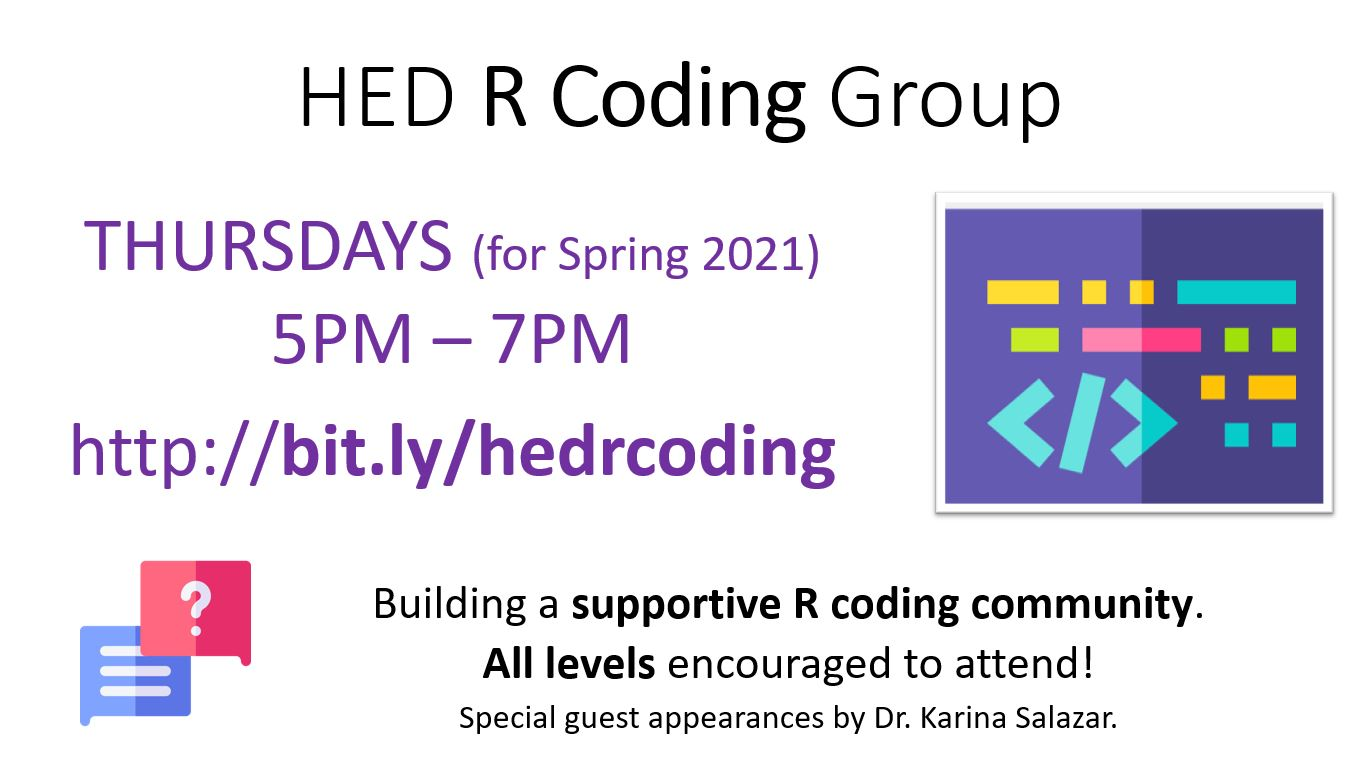
\includegraphics{hedrgroup.jpg}

\end{frame}

\begin{frame}{Today and Next Week}
\protect\hypertarget{today-and-next-week}{}

\textbf{Today}

\begin{itemize}
\tightlist
\item
  Intro to Bivariate Regression

  \begin{itemize}
  \tightlist
  \item
    linear regression model
  \item
    estimating parameters
  \end{itemize}
\end{itemize}

\medskip

\textbf{HW \& Reading}

\begin{itemize}
\tightlist
\item
  HW\#4 posted on D2L
\item
  Stock \& Watson Ch. 4 {[}finish if you haven't{]}
\end{itemize}

\medskip

\textbf{Next Week}

\begin{itemize}
\tightlist
\item
  Bivariate regression

  \begin{itemize}
  \tightlist
  \item
    Prediction
  \item
    Model fit
  \end{itemize}
\end{itemize}

\end{frame}

\hypertarget{introduction-to-bivariate-regression}{%
\section{Introduction to Bivariate
Regression}\label{introduction-to-bivariate-regression}}

\begin{frame}{Purpose of Regression}
\protect\hypertarget{purpose-of-regression}{}

\begin{itemize}
\item
  Regression analysis is a statistical method that helps us analyze and
  understand the relationship between 2+ variables
\item
  What is the purpose of regression in \textbf{descriptive research}
  (sometimes called ``observational studies'' or ``predictive''
  studies)?

  \begin{itemize}
  \tightlist
  \item
    To understand \textbf{relationship(s)} between one dependent
    variable (Y) to one or more indepedent variable (X, Z, etc.)
  \item
    Not concerned with ``direction'' or ``cause'': Does X cause Y? Does
    Y cause X?
  \item
    Interested in ``prediction''
  \item
    Example: predict poverty status based on having a cell phone
  \end{itemize}
\end{itemize}

\medskip

\begin{itemize}
\item
  What is the purpose of regression in \textbf{econometrics research}
  (sometimes called ``causal studies'')?

  \begin{itemize}
  \tightlist
  \item
    To estimate the \textbf{causal} effect of an independent variable
    (X) on a dependent variable (Y)
  \item
    Very concerned with ``direction'' or ``cause'': Does X cause Y?\\
  \item
    Interested in recreating experimental conditions or what would have
    happened under a randomized control trial
  \item
    Example: What is the effect of class size on student learning?
  \end{itemize}
\end{itemize}

\medskip

\begin{itemize}
\tightlist
\item
  Most of my research is descriptive; but I teach this class in a
  ``causal'' way\ldots{} why?

  \begin{itemize}
  \tightlist
  \item
    One type of research is not better than the other; it's just really
    important to understand the difference. \emph{Ex: Lack of a cell
    phone doesn't cause poverty!}
  \item
    Causal research forces you to be very purposeful about your models!
  \item
    Policy makers/decision makers don't just care if there is a
    relationship between class size and student learning; they want to
    know if we decrease class size by two students what is the expected
    change in student test scores
  \end{itemize}
\end{itemize}

\end{frame}

\begin{frame}{Regression: Models, Variables, Relationships}
\protect\hypertarget{regression-models-variables-relationships}{}

\begin{itemize}
\tightlist
\item
  \textbf{Linear Regression Model vs Non-Linear Regression Models}

  \begin{itemize}
  \tightlist
  \item
    Linear regression model (general linear model)

    \begin{itemize}
    \tightlist
    \item
      the dependent variable is continuous
    \item
      e.g., GPA, test scores, income
    \item
      \textbf{the focus of this class!}
    \end{itemize}
  \item
    Non-linear regression models (logit, ordinal, probit, poisson,
    negative binomial)

    \begin{itemize}
    \tightlist
    \item
      the dependent variable is non-continuous (i.e., categorical,
      binary, counts)
    \item
      e.g., persistence, likert scales, type of major
    \item
      \textbf{focus of HED 613} (Spring 2022/Maybe Fall 2021)
    \end{itemize}
  \end{itemize}
\end{itemize}

\medskip

\begin{itemize}
\tightlist
\item
  \textbf{Bivariate vs Multivariate Regression}

  \begin{itemize}
  \tightlist
  \item
    Bivariate regression (sometimes also called univariate, simple
    regression)

    \begin{itemize}
    \tightlist
    \item
      One dependent variable (Y) and one independent variable of
      interest (\(X_1\))
    \end{itemize}
  \item
    Multivariate regression (for econometrics/causal inference)

    \begin{itemize}
    \tightlist
    \item
      One dependent variable (Y) and one independent variable of
      interest (\(X_1\)); \textbf{and} multiple control variables
      (\(X_2\),\(X_3\),\(X_4\),etc.)
    \end{itemize}
  \end{itemize}
\end{itemize}

\medskip

\begin{itemize}
\tightlist
\item
  \textbf{Linear Relationship vs Non-Linear Relationship between X and
  Y}

  \begin{itemize}
  \tightlist
  \item
    Draw linear vs non-linear relationship scatterplots; show in R
  \item
    We will focus on modeling linear relationship between X and Y for
    first half of the course
  \item
    Then we will cover non-linear relationships
  \end{itemize}
\end{itemize}

\end{frame}

\begin{frame}[fragile]{Rest of Lecture: Same Example as Last Week}
\protect\hypertarget{rest-of-lecture-same-example-as-last-week}{}

\begin{itemize}
\tightlist
\item
  We will be using the same example as last week:

  \begin{itemize}
  \tightlist
  \item
    What is the effect of hours worked (X) on income (Y)?
  \end{itemize}
\end{itemize}

\medskip

\begin{itemize}
\tightlist
\item
  We'll be using the continuous version of income from PS3

  \begin{itemize}
  \tightlist
  \item
    \texttt{realrinc}
  \end{itemize}
\end{itemize}

\end{frame}

\begin{frame}{Slope Measures relationship between X and Y}
\protect\hypertarget{slope-measures-relationship-between-x-and-y}{}

\begin{itemize}
\tightlist
\item
  Research Question

  \begin{itemize}
  \tightlist
  \item
    What is the effect of hours worked (X) on annual income (Y)
  \end{itemize}
\end{itemize}

\medskip

\begin{itemize}
\tightlist
\item
  What do we want to measure?

  \begin{itemize}
  \tightlist
  \item
    The relationship between hours worked (X) and income (Y)
  \item
    If we increase the number of hours worked per week by one additional
    hour, how much do we expect annual income to change?
  \end{itemize}
\end{itemize}

\medskip

\begin{itemize}
\tightlist
\item
  We want to measure \(\beta\)

  \begin{itemize}
  \tightlist
  \item
    \(\beta = \frac{(Y_2 - Y_1)}{(X_2 - X_1)} = \frac{\Delta Y}{\Delta X}\)
  \item
    In other words, the slope of the relationship between X and Y
  \item
    Under the assumption of a linear relationship
  \end{itemize}
\end{itemize}

\medskip

\begin{itemize}
\tightlist
\item
  Draw line showing linear relationship between X and Y

  \begin{itemize}
  \tightlist
  \item
    \(x_1 = 31, x_2 =32, y_1=\$30,000, Y_2=\$35,000\)
  \item
    Calculate slope at different points and for different \(\Delta X\)
  \end{itemize}
\end{itemize}

\end{frame}

\hypertarget{population-linear-regression-model}{%
\subsection{Population Linear Regression
Model}\label{population-linear-regression-model}}

\begin{frame}{Population Linear Regression Model}
\protect\hypertarget{population-linear-regression-model-1}{}

\textbf{Population} Linear Regression Model

\begin{itemize}
\tightlist
\item
  \(Y_i = \beta_0 + \beta_1X_i + u_i\)
\end{itemize}

\medskip

Where:

\begin{itemize}
\tightlist
\item
  \(Y_i\) = income for person i
\item
  \(X_i\) = hours worked per week for person i
\item
  \(\beta_0\) (``population intercept'') = average income for someone
  with X=0
\item
  \(\beta_1\) (``population regression coefficient'') = average effect
  of a one-unit increase in X on the value of Y
\item
  \(u_1\) (``error term'' or ``residual'') = all other variables not
  included in your model that affect the value of Y
\end{itemize}

\medskip

Draw Picture

\begin{itemize}
\tightlist
\item
  Scatterplot of the population
\item
  Population regression model line
\item
  Label the following:

  \begin{itemize}
  \tightlist
  \item
    \(\beta_0\)
  \item
    \(\beta_1\)
  \item
    residual (predicted - value of \(Y_i\))
  \end{itemize}
\end{itemize}

\end{frame}

\begin{frame}{Population Regression Model}
\protect\hypertarget{population-regression-model}{}

\textbf{Population} Linear Regression Model
\(Y_i = \beta_0 + \beta_1X_i + u_i\)

\medskip

Contains two population parameters

\begin{itemize}
\tightlist
\item
  \(\beta_0\) (``population intercept'') = average income for someone
  with X=0
\item
  \(\beta_1\) (``population regression coefficient'') = average effect
  of a one-unit increase in X on the value of Y
\end{itemize}

\medskip

\begin{itemize}
\tightlist
\item
  How do we know these are population parameters? (hint: notation)
\item
  Do we usually know the value of \(\beta_0\) or \(\beta_1\)?
\end{itemize}

\end{frame}

\begin{frame}{Population regression coefficient, \(\beta_1\)}
\protect\hypertarget{population-regression-coefficient-beta_1}{}

What is the effect of hours worked per week (X) on income (Y)?

\begin{itemize}
\tightlist
\item
  Answer: population regression coefficient, \(\beta_1\)
\item
  Estimating \(\beta_1\) is the fundamental goal of causal
  inference/this course
\end{itemize}

\medskip

What is the population regression coefficient, \(\beta_1\)?

\begin{itemize}
\item
  \(\beta_1\) measures the average change in Y for a one-unit increase
  in X
\item
  Think of \(\beta_1\) as measuring the slope of our prediction line!
\item
  \(\beta_1 = \frac{\Delta Y}{\Delta X} = \frac{\Delta Income}{\Delta Hours Worked}\)
\item
  Example: \(\beta_1\) =
  \(\frac{\$5000 \Delta Income}{1hour \Delta HoursWorked}\) = \$5,000
\end{itemize}

\medskip

Interpretation (we will use this all semester!)

\begin{itemize}
\tightlist
\item
  General interpretation:

  \begin{itemize}
  \tightlist
  \item
    On average, a one unit-increase in X is associated with a
    \(\beta_1\) increase (or decrease) in the value of Y
  \end{itemize}
\item
  Interpretation from example above:

  \begin{itemize}
  \tightlist
  \item
    On average, a one-hour increase in hours worked per week (X) is
    associated with a \$5,000 (\(\beta_1\)) increase in annual income
    (Y)
  \end{itemize}
\item
  Interpret if \(\beta_1 = \$2,000\); or \(\beta_1 = \$4,000\)
\end{itemize}

\end{frame}

\begin{frame}{Population regression coefficient, \(\beta_1\)}
\protect\hypertarget{population-regression-coefficient-beta_1-1}{}

Some important things to remember:

\begin{itemize}
\item
  If \(\beta_1\) (i.e., the relationship between X and Y) is linear,
  then the average change in Y for a one-unit increase in X is the same
  no matter the starting value of X

  \begin{itemize}
  \tightlist
  \item
    Like plot example from earlier
  \end{itemize}
\item
  \(\beta_1\) measures the \textbf{average} effect on Y for a one-unit
  increase in X; this effect on an individual observation may be
  different than this average effect!
\item
  \(\beta_1\) is a population parameter. We hardly ever know population
  parameters. So we \textbf{estimate} \(\beta_1\) using sample data!
\end{itemize}

\end{frame}

\begin{frame}{Population Intercept, \(\beta_0\)}
\protect\hypertarget{population-intercept-beta_0}{}

What is the effect of hours worked per week (X) on annual income (Y)?

\begin{itemize}
\tightlist
\item
  \(Y_i = \beta_0 + \beta_1X_i + u_i\)
\end{itemize}

\medskip

\(\beta_0\) is the ``population intercept''

\begin{itemize}
\tightlist
\item
  \(\beta_0\) = the average value of Y when X=0
\item
  Here, \(\beta_0\), is the average annual income for someone that works
  zero hours per week (X=0)
\item
  Usually, we are not substantively interested in \(\beta_0\)
\item
  Sometimes \(\beta_0\) is non-sensical or there's too few observations
  at X=0 to calculate a precise estimate (e.g., effect of age on income)
\end{itemize}

\end{frame}

\hypertarget{population-linear-regression-line}{%
\subsection{Population Linear Regression
Line}\label{population-linear-regression-line}}

\begin{frame}{Population Linear Regression \emph{LINE}}
\protect\hypertarget{population-linear-regression-line-1}{}

\textbf{Population} Linear Regression Model
\(Y_i = \beta_0 + \beta_1X_i + u_i\)

\medskip

We sometimes deconstruct the Population Linear Regression Model into two
parts:

\begin{enumerate}
[(1)]
\tightlist
\item
  \textbf{Population} Linear Regression \emph{LINE}/ Regression
  Function: \(Y_i = \beta_0 + \beta_1X_i\)
\item
  \textbf{Population} ``Error'' or ``Residual'' Term: \(u_i\)
\end{enumerate}

\medskip

\begin{itemize}
\tightlist
\item
  Population regression line: just a linear prediction line, like the
  one in the scatterplot \emph{if} the scatterplot contained all
  observation in the population
\item
  Population regression line measures the ``average'' or ``expected''
  relationship between X and Y, ignoring variables that we excluded from
  the model (i.e., \(u_i\))
\end{itemize}

\end{frame}

\begin{frame}{Population Linear Regression \emph{LINE}}
\protect\hypertarget{population-linear-regression-line-2}{}

Population regression line and Expected Value, E(Y)

\begin{itemize}
\tightlist
\item
  Expected value of Y (for a sample mean/ one variable)

  \begin{itemize}
  \tightlist
  \item
    \(E(Y) = \mu_Y\)
  \end{itemize}
\end{itemize}

\medskip

\begin{itemize}
\tightlist
\item
  Expected value of Y, given the value of X (relationship between two
  variables)

  \begin{itemize}
  \tightlist
  \item
    \(E(Y|X) = \beta_0 + \beta_1X_i\)
  \item
    the population regression line is expected value of Y for a given
    value of X
  \end{itemize}
\end{itemize}

\medskip

\begin{itemize}
\tightlist
\item
  Population regression line and prediction

  \begin{itemize}
  \item
    If we know value of parameters, \(\beta_0\) and \(\beta_1\), we can
    predict value of Y
  \item
    Example: \(\beta_0=\$5,000\) and \(\beta_1=\$2,000\)
  \item
    \begin{enumerate}
    [(1)]
    \tightlist
    \item
      Predict the value of Y (annual income) for someone that works 20
      hours per week
    \end{enumerate}
  \item
    \begin{enumerate}
    [(1)]
    \setcounter{enumi}{1}
    \tightlist
    \item
      Predict the value of Y (annual income) for someone that works 45
      hours per week
    \end{enumerate}
  \end{itemize}
\end{itemize}

\end{frame}

\begin{frame}{\(u_i\) as ``Error Term''}
\protect\hypertarget{u_i-as-error-term}{}

\begin{itemize}
\tightlist
\item
  Population linear regression model

  \begin{itemize}
  \tightlist
  \item
    \(Y_i = \beta_0 + \beta_1X_i + u_i\)
  \item
    Y= income; \(X_i\)= hours worked
  \end{itemize}
\end{itemize}

\medskip

\begin{itemize}
\tightlist
\item
  In causal inference research:

  \begin{itemize}
  \tightlist
  \item
    Error term \(u_i\) represents (consists of) \emph{all other
    variables besides X that are not included in your model} that affect
    the dependent variable
  \item
    In other words, the error term consists of all other factors (i.e.,
    variables) responsible for the difference between the \(i^{th}\)
    district's average test score and the value predicted by the
    regression line
  \item
    This interpretation will become \emph{super} important down the
    road!
  \end{itemize}
\end{itemize}

\medskip

\begin{itemize}
\tightlist
\item
  Example of Y= income; \(X_i\)= hours worked; the error term \(u_i\)
  would consist of other factors besides hours worked that have an
  effect on yearly income!

  \begin{itemize}
  \tightlist
  \item
    Occupation: a hedge fund manager can 20 hours a week and make
    millions (maybe not last week tho!); an essential worker can 80+
    hours and still only \$40k
  \item
    Race: BIPOC face discrimination in labor wages
  \item
    Gender pay gap!
  \end{itemize}
\end{itemize}

\medskip

\begin{itemize}
\tightlist
\item
  In other social science based statistics classes

  \begin{itemize}
  \tightlist
  \item
    Interpret the \(u_i\) as the overall error in the prediction of Y
    due to \emph{random variation}
  \end{itemize}
\end{itemize}

\end{frame}

\begin{frame}{\(u_i\) as ``Residual''}
\protect\hypertarget{u_i-as-residual}{}

\begin{itemize}
\tightlist
\item
  Population linear regression model

  \begin{itemize}
  \tightlist
  \item
    \(Y_i = \beta_0 + \beta_1X_i + u_i\)
  \item
    Y= income; \(X_i\)= hours worked
  \end{itemize}
\end{itemize}

\medskip

\begin{itemize}
\tightlist
\item
  \(u_i\) as the residual

  \begin{itemize}
  \tightlist
  \item
    Population regression line represents the predicted value of Y
    (income) for each value of X (hours worked)
  \item
    Residual = the predicted value of Y - observed value of Y for any
    given value of X
  \end{itemize}
\end{itemize}

\medskip

\begin{itemize}
\item
  Easier to conceptually think about \(u_i\) in terms of each
  observation, i

  \begin{itemize}
  \tightlist
  \item
    \(Y_i\) = actual value of income for person i
  \item
    \(Y_i = \beta_0 + \beta_1X_i\) = Population Regression line

    \begin{itemize}
    \tightlist
    \item
      The predicted value of income for person i with hours worked =
      \(X_i\)
    \end{itemize}
  \item
    Residual, \(u_i\)

    \begin{itemize}
    \tightlist
    \item
      The difference between actual value, \(Y_i\), and predicted value
      from the population regression line for observation i
    \item
      \(u_i = Y_i - (\beta_0 + \beta_1X_i)\)
    \end{itemize}
  \end{itemize}
\end{itemize}

\end{frame}

\hypertarget{break-5-10-min}{%
\subsection{BREAK {[}5-10 min{]}}\label{break-5-10-min}}

\hypertarget{estimating-regression-parameters}{%
\subsection{Estimating Regression
Parameters}\label{estimating-regression-parameters}}

\begin{frame}{General things we do in regression analysis}
\protect\hypertarget{general-things-we-do-in-regression-analysis}{}

\begin{enumerate}
\tightlist
\item
  \textbf{Estimation} {[}Today{]}
\end{enumerate}

\begin{itemize}
\tightlist
\item
  How do we choose estimates of \(\beta_0\) and \(\beta_1\) using sample
  data?
\end{itemize}

\medskip

\begin{enumerate}
\setcounter{enumi}{1}
\tightlist
\item
  \textbf{Prediction} {[}Next Week{]}
\end{enumerate}

\begin{itemize}
\tightlist
\item
  What is the predicted value of Y for someone with a particular value
  of X?
\end{itemize}

\medskip

\begin{enumerate}
\setcounter{enumi}{2}
\tightlist
\item
  \textbf{Hypothesis testing} {[}focus of the rest of the semester{]}
\end{enumerate}

\begin{itemize}
\tightlist
\item
  Hypothesis testing and confidence intervals about \(\beta_1\)
\end{itemize}

\end{frame}

\begin{frame}{Step 1 of regression: Estimate Parameters}
\protect\hypertarget{step-1-of-regression-estimate-parameters}{}

Population linear regression model

\begin{itemize}
\tightlist
\item
  \(Y_i = \beta_0 + \beta_1X_i + u_i\)
\end{itemize}

\medskip

\textbf{Goal of estimation is to}:

\begin{itemize}
\tightlist
\item
  Use sample data to estimate the population intercept, \(\beta_0\), and
  the population regression coefficient, \(\beta_1\)
\item
  \(\hat{\beta_0}\) is an estimate of \(\beta_0\)
\item
  \(\hat{\beta_1}\) is an estimate of \(\beta_1\)

  \begin{itemize}
  \tightlist
  \item
    How dow we know these estimates are based on sample data and not
    population parameters? (hint: notation!)
  \end{itemize}
\end{itemize}

\medskip

\textbf{Estimation problem}:

Need to develop a method for choosing values of \(\hat{\beta_0}\) and
\(\hat{\beta_1}\)

\end{frame}

\begin{frame}{Estimation (population mean)}
\protect\hypertarget{estimation-population-mean}{}

We faced a similar estimation problem in intro to stats!

\begin{itemize}
\tightlist
\item
  Use sample to calculate the ``best'' estimate of the population mean,
  \(\mu_Y\)
\item
  We decided sample mean, \(\bar{Y}\), was the ``best'' estimate!
\end{itemize}

\medskip

Criteria we used to determine \(\bar{Y}\) was ``best'' estimate of
\(\mu_Y\)

\begin{itemize}
\tightlist
\item
  \(m\) is all potential estimates for \(\mu_Y\)
\item
  Goal: choose the value, \(m\) , that minimizes the ``sum of squares''

  \begin{itemize}
  \tightlist
  \item
    Sum of squares = \(\sum_{i=1}^{n}\) \((Y_i-m)^2\)
  \item
    \(\bar{Y}\) is the value of \(m\) that minimizes sum of squares
  \item
    So \(\bar{Y}\) is the ``least squares'' estimator
  \end{itemize}
\end{itemize}

\medskip

Draw scatterplot:

\begin{itemize}
\item
  \begin{enumerate}
  [(1)]
  \tightlist
  \item
    Horizontal line representing sample mean
  \end{enumerate}

  \begin{itemize}
  \tightlist
  \item
    Show formula for sum of square errors
  \end{itemize}
\end{itemize}

\end{frame}

\begin{frame}{Estimation (regression)}
\protect\hypertarget{estimation-regression}{}

Problem in regression:

\begin{itemize}
\tightlist
\item
  Need to develop method for selecting the ``best'' estimate of
  \(\hat{\beta_0}\) and \(\hat{\beta_1}\)
\item
  Solution: similar to what we do for population mean!
\end{itemize}

\medskip

First some terminology:

\begin{itemize}
\tightlist
\item
  \(Y_i\) is the actual observed value of Y for individual i
\item
  \(\hat{Y_i}\) is the predicted value of \(Y_i\), based on sample data!

  \begin{itemize}
  \tightlist
  \item
    \(\hat{Y_i} = \hat{\beta_0} + \hat{\beta_1}X_i\)
  \end{itemize}
\item
  Estimated residual, \(\hat{u}_i\) is the difference between actual
  \(Y_i\) and predicted \(\hat{Y_i}\)

  \begin{itemize}
  \tightlist
  \item
    \(Y_i - \hat{Y_i}\) = \(\hat{u_i}\)
  \item
    \(Y_i - (\hat{\beta_0} + \hat{\beta_1}X_i)\) = \(\hat{u_i}\)
  \item
    Residuals are sometimes called ``errors''
  \end{itemize}
\end{itemize}

\end{frame}

\begin{frame}{Estimation (regression)}
\protect\hypertarget{estimation-regression-1}{}

Criteria for choosing ``best'' estimate of \(\hat{\beta_0}\) and
\(\hat{\beta_1}\)

\begin{itemize}
\tightlist
\item
  Select values that minimize ``sum of squared residuals''
\end{itemize}

\medskip

Sum of squared residuals (or sometimes called ``sum of squared
errors''):

\begin{itemize}
\item
  \(\sum_{i=1}^{n}\) \((Y_i - \hat{Y_i})^2\)
\item
  \(\sum_{i=1}^{n}\) \((Y_i - (\hat{\beta_0} + \hat{\beta_1}X_i))^2\)
\item
  \(\sum_{i=1}^{n}\) \((u_i)^2\)
\end{itemize}

\medskip

\textbf{Ordinary Least Squares} is a linear method for estimating
parameters in a linear regression model

\begin{itemize}
\tightlist
\item
  Method draws a line through the sample data points that minimizes the
  sum of squared residuals, or in other words, the differences between
  the observed values and the corresponding fitted values
\item
  Minimization is achieved via calculus (derivatives). R will calculate
  this for you (phew!)
\item
  Best estimates of \(\hat{\beta_0}\) and \(\hat{\beta_1}\) are those
  that any other alternatives would result in a higher sum of squared
  residuals
\end{itemize}

\end{frame}

\begin{frame}{OLS Prediction Line}
\protect\hypertarget{ols-prediction-line}{}

\textbf{Population Linear Regression Model}

\begin{itemize}
\tightlist
\item
  \(Y_i = \beta_0 + \beta_1X_i + u_i\)
\end{itemize}

\medskip

\textbf{OLS Prediction Line or ``OLS Regression Line'' (based on sample
data)}

\begin{itemize}
\tightlist
\item
  \(\hat{Y_i} = \hat{\beta_0} + \hat{\beta_1}X_i\)
\end{itemize}

\medskip

\begin{itemize}
\tightlist
\item
  Our OLS prediction line chose the best estimates of \(\hat{\beta_0}\)
  and \(\hat{\beta_1}\) as those that any other alternatives would
  result in a higher sum of squared residuals
\item
  Draw this out\ldots{}
\end{itemize}

\end{frame}

\begin{frame}[fragile]{Let's write run our first regression and write
out our models!}
\protect\hypertarget{lets-write-run-our-first-regression-and-write-out-our-models}{}

RQ: What is the effect of hours worked per week on annual income?

\begin{itemize}
\tightlist
\item
  Run regression in R

  \begin{itemize}
  \tightlist
  \item
    \texttt{mod1\ \textless{}-\ lm(realrinc\ \textasciitilde{}\ hrs1,\ data=gss)}
  \item
    \texttt{summary(mod1)}
  \end{itemize}
\end{itemize}

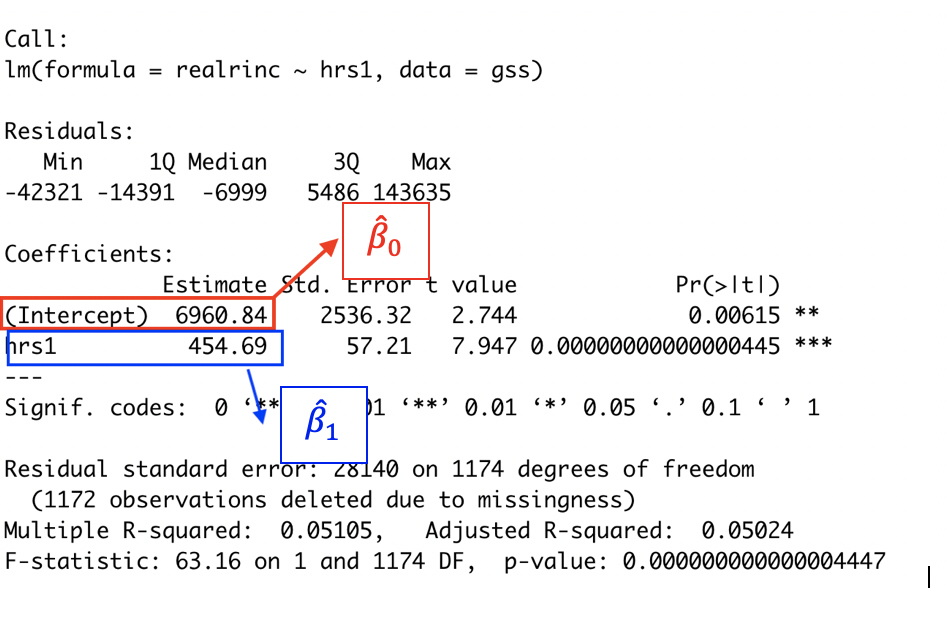
\includegraphics{output.png}

\end{frame}

\begin{frame}{Let's write run our first regression and write out our
models!}
\protect\hypertarget{lets-write-run-our-first-regression-and-write-out-our-models-1}{}

RQ: What is the effect of hours worked per week on annual income?

\medskip

Write out and label everything within the following: {[}we will be doing
this all semester!{]}

\begin{enumerate}
\tightlist
\item
  Population regression model

  \begin{itemize}
  \tightlist
  \item
    Label Y; Label X
  \end{itemize}
\item
  OLS Prediction Line (without estimates)

  \begin{itemize}
  \tightlist
  \item
    Define \(\hat{\beta_0}\)?
  \item
    Define \(\hat{\beta_1}\)?
  \end{itemize}
\item
  OLS Prediction Line (with estimates)

  \begin{itemize}
  \tightlist
  \item
    Interpret \(\hat{\beta_0}\) given the estimate
  \item
    Interpret \(\hat{\beta_1}\) given the estimate
  \end{itemize}
\item
  Predict the expected value of \(\hat{Y}_i\) for someone that works 60
  hours a week.
\end{enumerate}

\end{frame}

\begin{frame}[fragile]{In-Class Group Exercise}
\protect\hypertarget{in-class-group-exercise}{}

RQ: What is the effect of age on annual income??

\begin{itemize}
\tightlist
\item
  hint! X = \texttt{age} and Y =\texttt{realrinc}
\end{itemize}

\medskip

Write out and label everything within the following

\begin{itemize}
\tightlist
\item
  Recommendation: Practice how to write out equations in Word;
  touch-screen devices share your screen via whiteboard
\end{itemize}

\begin{enumerate}
\tightlist
\item
  Population regression model

  \begin{itemize}
  \tightlist
  \item
    Label Y; Label X
  \end{itemize}
\item
  OLS Prediction Line (without estimates)

  \begin{itemize}
  \tightlist
  \item
    Define \(\hat{\beta_0}\)?
  \item
    Define \(\hat{\beta_1}\)?
  \end{itemize}
\item
  OLS Prediction Line (with estimates)

  \begin{itemize}
  \tightlist
  \item
    Run regression in R and print to get estimates:

    \begin{itemize}
    \tightlist
    \item
      \texttt{mod2\ \textless{}-\ \ lm(realrinc\ \textasciitilde{}\ age,\ data=gss)}
    \item
      \texttt{summary(mod2)}
    \end{itemize}
  \item
    Interpret \(\hat{\beta_0}\) given the estimate
  \item
    Interpret \(\hat{\beta_1}\) given the estimate
  \end{itemize}
\item
  Predict the expected value of \(\hat{Y}_i\) for someone that is 18
  years old.
\end{enumerate}

\end{frame}

\begin{frame}{In-Class Group Exercise {[}Solutions{]}}
\protect\hypertarget{in-class-group-exercise-solutions}{}

RQ: What is the effect of age on annual income??

\begin{enumerate}
\tightlist
\item
  Population regression model

  \begin{itemize}
  \tightlist
  \item
    \(Y_i = \beta_0 + \beta_1X_i + u_i\)
  \item
    Y = annual income; X = age
  \end{itemize}
\item
  OLS Prediction Line (without estimates)

  \begin{itemize}
  \tightlist
  \item
    \(\hat{Y_i} = \hat{\beta_0} + \hat{\beta_1}X_i\)
  \item
    \(\hat{\beta_0}\)? = Sample population intercept

    \begin{itemize}
    \tightlist
    \item
      i.e., the average value of Y when X=0
    \end{itemize}
  \item
    \(\hat{\beta_1}\) = Sample regression coefficient

    \begin{itemize}
    \tightlist
    \item
      i.e., the average change in Y for one-unit increase in X
    \end{itemize}
  \end{itemize}
\item
  OLS Prediction Line (with estimates)

  \begin{itemize}
  \tightlist
  \item
    \(\hat{Y_i} = \$8,620 + \$368X_i\)
  \item
    \(\hat{\beta_0}\) = \$8,620

    \begin{itemize}
    \tightlist
    \item
      On average, someone who is age zero has an annual income of
      \$8,620
    \item
      Example of non-sensical \(\hat{\beta_0}\)
    \end{itemize}
  \item
    \(\hat{\beta_1}\)? = \$368

    \begin{itemize}
    \tightlist
    \item
      On average, a one-year increase in age is associated with a \$368
      increase in annual income
    \end{itemize}
  \end{itemize}
\item
  Predict the expected value of \(\hat{Y}_i\) for someone that is 18
  years old.

  \begin{itemize}
  \tightlist
  \item
    \(E(\hat{Y_i}|X=35)\) = \(\hat{Y_i} = \$8,620 + \$368*18\)
  \item
    \(E(\hat{Y_i}|X=35)\) = \(\hat{Y_i} = \$8,620 + \$6,624\)
  \item
    \(E(\hat{Y_i}|X=35)\) = \$15,244
  \end{itemize}
\end{enumerate}

\end{frame}

\end{document}
